Os questionários são submetidos aos alunos e especialistas para coletar os dados necessários para análise. Qualquer dificuldade ou problema encontrado para se enviar determinado dado deverá ser comunicado para evitar análises incorretas, com dados inválidos. Dados redundantes vindos de uma mesma pessoa devem ser considerados apenas uma vez, por isso o número de respostas dos questionários está limitado a uma resposta por pessoa. Os indivíduos terão suas identidades resguardadas de modo a não expô-los.%, uma vez que o objetivo do estudo não é este.

Com os questionários, espera-se estipular valores para as seguintes métricas: i) satisfação dos alunos com as atividades práticas; ii) satisfação do professor com o progresso da turma; iii) relação das atividades com o mercado; iv) taxa de mudança da satisfação dos alunos com as atividades; v) taxa de mudança da satisfação do professor com as atividades. Tais métricas são usadas para a análise dos possíveis benefícios com o uso da etapa de \textit{Measure} do \textit{Lean Learning}. O uso da escala tipo Likert de cinco pontos possibilitou a obtenção de uma graduação quantificada das percepções dos entrevistados\cite{marconi2003fundamentos}.O maior benefício da escala Likert é conseguir medir, de forma graduada, graus de concordância ou não a um conjunto de afirmativas.

A cada questionário aberto, busca-se analisar indícios de convergência em uma ideia ou opinião, baseado nos métodos propostos nos trabalhos de Bandeira (2003) e Henkel (2017), conforme o número de respostas semelhantes. Os dados dos questionários abertos e fechados são comparados a fim de verificar se apresentam resultados coerentes entre si e os resultados são repassados ao especialista relacionado, conforme mencionado anteriormente. O especialista, por sua vez, busca identificar possibilidades de melhoria constante, como prevê o \textit{Lean}, e propõe uma abordagem nova, que busque valorizar os pontos que despertaram interesse nos alunos.

\begin{figure}
    \centering
    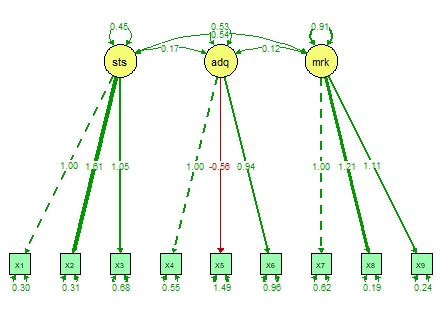
\includegraphics[width=13cm,height=7cm]{Imagens/RPlot.jpg}
    \caption{Plot}
    \label{fig:Plot}
\end{figure}

Foram recolhidas 68 respostas nos questionários de \textit{feedback} sobre as atividades, sendo assim, uma amostra viável para a concretização desse estudo, visto que o número mínimo necessário seriam de 50 respostas \cite{hair2009analise}. A partir dessas respostas e da análise do algoritmo em R, observa-se que a satisfação dos alunos e a proximidade com o mercado estão em níveis satisfatórios. Em contrapartida, a adequação das práticas precisa ser melhorada, principalmente em questão de tempo. %talvez tal discrepância nas respostas seja devido ao fato de várias turmas de períodos diferentes estarem fazendo a mesma prática.

Ainda assim os resultados apresentaram uma forte correlação entre as perguntas referente a satisfação dos alunos e também quando a proximidade ao mercado, mostrando que o \textit{Lean Learning} pode sim ser uma metodologia de ensino que prepara melhor os alunos para as atividades comerciais de \textit{software}. Para melhorar ainda mais seu desempenho, precisaria se adequar melhor cada atividade prática para cada turma do curso, baseando no nível da turma, período e complexidade envolvida.

Tais afirmações foram feitas baseadas no resultado do CFA e do teste T obtidos através do algoritmo descrito no apêndice desse trabalho. O nível de significância $\alpha$1 utilizado neste estudo é de 0,05 (intervalo de confiança de 95\%). No entanto, ainda poder-se-ia aceitar $\alpha$=0,10 \cite{hair2009analise}. Observamos que o \textit{Alpha de Cronbach} nas variáveis de satisfação e mercado atingiu um nível adequado, sendo o de satisfação um valor de 0,79 e o de mercado um valor de 0,9. Enquanto a variável de adequação ainda precisaria de melhorias, visto que foi obtido uma confiabilidade de 0,3 apenas.

A correlação entre as variáveis existiu apenas entre a variável de satisfação e de mercado, essas tendo um resultado de p < 0,05. A variável de adequação não apresenta correlação devido ao fato de que ela mesma não pode carregar confiabilidade em suas respostas e portanto, apresentou um valor p em relação as outras variáveis maior que 0,05.